\documentclass{standalone}
\usepackage{tikz}
\usetikzlibrary{patterns, positioning}

\begin{document}
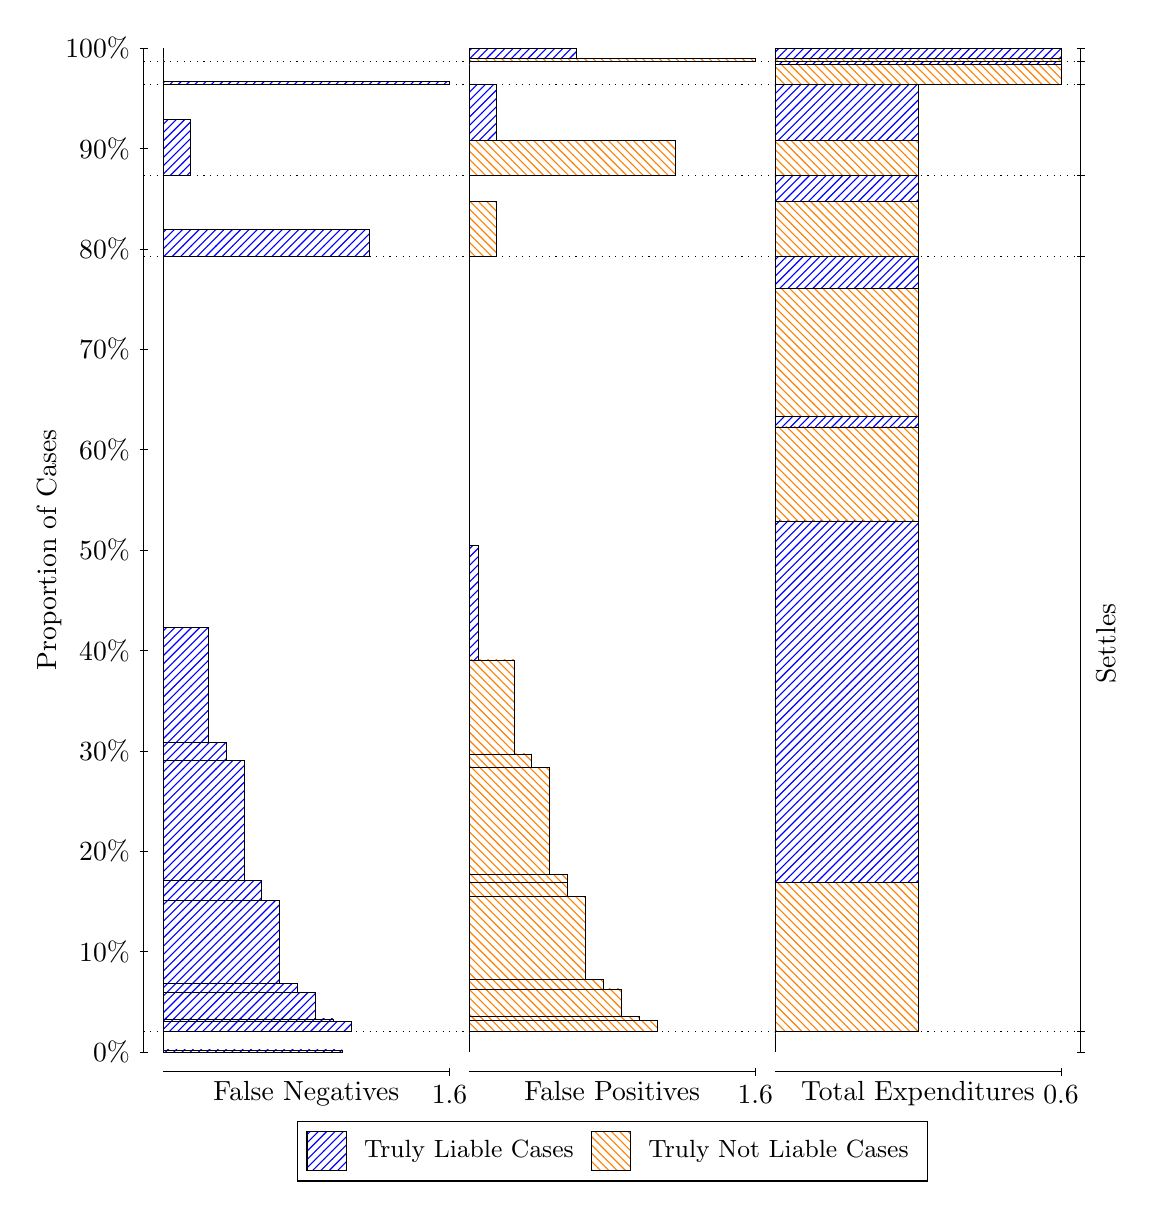
\begin{tikzpicture}
\draw[black, very thin] (1.5,1.75) -- (1.5,14.5);
\node[rotate=90, anchor=center] at (0.3, 8.125) {Proportion of Cases};
\draw[black, very thin] (1.45,1.75) -- (1.55,1.75);
\node[anchor=east] at (1.45, 1.75) {0\%};
\draw[black, very thin] (1.45,3.025) -- (1.55,3.025);
\node[anchor=east] at (1.45, 3.025) {10\%};
\draw[black, very thin] (1.45,4.3) -- (1.55,4.3);
\node[anchor=east] at (1.45, 4.3) {20\%};
\draw[black, very thin] (1.45,5.575) -- (1.55,5.575);
\node[anchor=east] at (1.45, 5.575) {30\%};
\draw[black, very thin] (1.45,6.85) -- (1.55,6.85);
\node[anchor=east] at (1.45, 6.85) {40\%};
\draw[black, very thin] (1.45,8.125) -- (1.55,8.125);
\node[anchor=east] at (1.45, 8.125) {50\%};
\draw[black, very thin] (1.45,9.4) -- (1.55,9.4);
\node[anchor=east] at (1.45, 9.4) {60\%};
\draw[black, very thin] (1.45,10.675) -- (1.55,10.675);
\node[anchor=east] at (1.45, 10.675) {70\%};
\draw[black, very thin] (1.45,11.95) -- (1.55,11.95);
\node[anchor=east] at (1.45, 11.95) {80\%};
\draw[black, very thin] (1.45,13.225) -- (1.55,13.225);
\node[anchor=east] at (1.45, 13.225) {90\%};
\draw[black, very thin] (1.45,14.5) -- (1.55,14.5);
\node[anchor=east] at (1.45, 14.5) {100\%};

\draw[black, very thin] (13.4,1.75) -- (13.4,14.5);
\draw[black, very thin] (13.35,1.75) -- (13.45,1.75);
\node[anchor=west] at (13.35, 1.75) {};
\draw[black, very thin] (13.35,2.0104) -- (13.45,2.0104);
\node[anchor=west] at (13.35, 2.0104) {};
\draw[black, very thin] (13.35,11.857) -- (13.45,11.857);
\node[anchor=west] at (13.35, 11.857) {};
\draw[black, very thin] (13.35,12.883) -- (13.45,12.883);
\node[anchor=west] at (13.35, 12.883) {};
\draw[black, very thin] (13.35,14.042) -- (13.45,14.042);
\node[anchor=west] at (13.35, 14.042) {};
\draw[black, very thin] (13.35,14.331) -- (13.45,14.331);
\node[anchor=west] at (13.35, 14.331) {};
\draw[black, very thin] (13.35,14.5) -- (13.45,14.5);
\node[anchor=west] at (13.35, 14.5) {};

\draw[black, very thin, pattern color=blue, pattern=north east lines] (1.75,1.75) rectangle (4.0208,1.7774);
\draw[black, very thin, pattern color=orange, pattern=north west lines] (1.75,1.7774) rectangle (1.75,2.0104);
\draw[black, very thin, pattern color=blue, pattern=north east lines] (1.75,2.0104) rectangle (4.1344,2.1409);
\draw[black, very thin, pattern color=blue, pattern=north east lines] (1.75,2.1409) rectangle (3.9073,2.1701);
\draw[black, very thin, pattern color=blue, pattern=north east lines] (1.75,2.1701) rectangle (3.6802,2.5078);
\draw[black, very thin, pattern color=blue, pattern=north east lines] (1.75,2.5078) rectangle (3.4531,2.6165);
\draw[black, very thin, pattern color=blue, pattern=north east lines] (1.75,2.6165) rectangle (3.226,3.6757);
\draw[black, very thin, pattern color=blue, pattern=north east lines] (1.75,3.6757) rectangle (2.999,3.9271);
\draw[black, very thin, pattern color=blue, pattern=north east lines] (1.75,3.9271) rectangle (2.7719,5.4502);
\draw[black, very thin, pattern color=blue, pattern=north east lines] (1.75,5.4502) rectangle (2.5448,5.6854);
\draw[black, very thin, pattern color=blue, pattern=north east lines] (1.75,5.6854) rectangle (2.3177,7.138);
\draw[black, very thin, pattern color=orange, pattern=north west lines] (1.75,7.138) rectangle (1.75,11.857);
\draw[black, very thin, pattern color=blue, pattern=north east lines] (1.75,11.857) rectangle (4.3615,12.192);
\draw[black, very thin, pattern color=orange, pattern=north west lines] (1.75,12.192) rectangle (1.75,12.883);
\draw[black, very thin, pattern color=blue, pattern=north east lines] (1.75,12.883) rectangle (2.0906,13.598);
\draw[black, very thin, pattern color=orange, pattern=north west lines] (1.75,13.598) rectangle (1.75,14.042);
\draw[black, very thin, pattern color=blue, pattern=north east lines] (1.75,14.042) rectangle (5.3833,14.081);
\draw[black, very thin, pattern color=orange, pattern=north west lines] (1.75,14.081) rectangle (1.75,14.331);
\draw[black, very thin, pattern color=orange, pattern=north west lines] (1.75,14.331) rectangle (1.75,14.369);
\draw[black, very thin, pattern color=blue, pattern=north east lines] (1.75,14.369) rectangle (1.75,14.5);
\draw[black, very thin, pattern color=orange, pattern=north west lines] (5.6333,1.75) rectangle (5.6333,1.983);
\draw[black, very thin, pattern color=blue, pattern=north east lines] (5.6333,1.983) rectangle (5.6333,2.0104);
\draw[black, very thin, pattern color=orange, pattern=north west lines] (5.6333,2.0104) rectangle (8.0177,2.1472);
\draw[black, very thin, pattern color=orange, pattern=north west lines] (5.6333,2.1472) rectangle (7.7906,2.2051);
\draw[black, very thin, pattern color=orange, pattern=north west lines] (5.6333,2.2051) rectangle (7.5635,2.5506);
\draw[black, very thin, pattern color=orange, pattern=north west lines] (5.6333,2.5506) rectangle (7.3365,2.6766);
\draw[black, very thin, pattern color=orange, pattern=north west lines] (5.6333,2.6766) rectangle (7.1094,3.7244);
\draw[black, very thin, pattern color=orange, pattern=north west lines] (5.6333,3.7244) rectangle (6.8823,3.9085);
\draw[black, very thin, pattern color=orange, pattern=north west lines] (5.6333,3.9085) rectangle (6.8823,4.0094);
\draw[black, very thin, pattern color=orange, pattern=north west lines] (5.6333,4.0094) rectangle (6.6552,5.3642);
\draw[black, very thin, pattern color=orange, pattern=north west lines] (5.6333,5.3642) rectangle (6.4281,5.5356);
\draw[black, very thin, pattern color=orange, pattern=north west lines] (5.6333,5.5356) rectangle (6.201,6.7294);
\draw[black, very thin, pattern color=blue, pattern=north east lines] (5.6333,6.7294) rectangle (5.7469,8.182);
\draw[black, very thin, pattern color=blue, pattern=north east lines] (5.6333,8.182) rectangle (5.6333,11.857);
\draw[black, very thin, pattern color=orange, pattern=north west lines] (5.6333,11.857) rectangle (5.974,12.548);
\draw[black, very thin, pattern color=blue, pattern=north east lines] (5.6333,12.548) rectangle (5.6333,12.883);
\draw[black, very thin, pattern color=orange, pattern=north west lines] (5.6333,12.883) rectangle (8.2448,13.327);
\draw[black, very thin, pattern color=blue, pattern=north east lines] (5.6333,13.327) rectangle (5.974,14.042);
\draw[black, very thin, pattern color=orange, pattern=north west lines] (5.6333,14.042) rectangle (5.6333,14.291);
\draw[black, very thin, pattern color=blue, pattern=north east lines] (5.6333,14.291) rectangle (5.6333,14.331);
\draw[black, very thin, pattern color=orange, pattern=north west lines] (5.6333,14.331) rectangle (9.2667,14.369);
\draw[black, very thin, pattern color=blue, pattern=north east lines] (5.6333,14.369) rectangle (6.9958,14.5);
\draw[black, very thin, pattern color=orange, pattern=north west lines] (9.5167,1.75) rectangle (9.5167,1.983);
\draw[black, very thin, pattern color=blue, pattern=north east lines] (9.5167,1.983) rectangle (9.5167,2.0104);
\draw[black, very thin, pattern color=orange, pattern=north west lines] (9.5167,2.0104) rectangle (11.333,3.9085);
\draw[black, very thin, pattern color=blue, pattern=north east lines] (9.5167,3.9085) rectangle (11.333,8.4952);
\draw[black, very thin, pattern color=orange, pattern=north west lines] (9.5167,8.4952) rectangle (11.333,9.689);
\draw[black, very thin, pattern color=blue, pattern=north east lines] (9.5167,9.689) rectangle (11.333,9.8195);
\draw[black, very thin, pattern color=orange, pattern=north west lines] (9.5167,9.8195) rectangle (11.333,11.447);
\draw[black, very thin, pattern color=blue, pattern=north east lines] (9.5167,11.447) rectangle (11.333,11.857);
\draw[black, very thin, pattern color=orange, pattern=north west lines] (9.5167,11.857) rectangle (11.333,12.548);
\draw[black, very thin, pattern color=blue, pattern=north east lines] (9.5167,12.548) rectangle (11.333,12.883);
\draw[black, very thin, pattern color=orange, pattern=north west lines] (9.5167,12.883) rectangle (11.333,13.327);
\draw[black, very thin, pattern color=blue, pattern=north east lines] (9.5167,13.327) rectangle (11.333,14.042);
\draw[black, very thin, pattern color=orange, pattern=north west lines] (9.5167,14.042) rectangle (13.15,14.291);
\draw[black, very thin, pattern color=blue, pattern=north east lines] (9.5167,14.291) rectangle (13.15,14.331);
\draw[black, very thin, pattern color=orange, pattern=north west lines] (9.5167,14.331) rectangle (13.15,14.369);
\draw[black, very thin, pattern color=blue, pattern=north east lines] (9.5167,14.369) rectangle (13.15,14.5);
\draw[black, dotted] (1.5,2.0104) -- (13.4,2.0104);
\draw[black, dotted] (1.5,11.857) -- (13.4,11.857);
\draw[black, dotted] (1.5,12.883) -- (13.4,12.883);
\draw[black, dotted] (1.5,14.042) -- (13.4,14.042);
\draw[black, dotted] (1.5,14.331) -- (13.4,14.331);
\draw[black, very thin] (1.75,1.5) -- (5.3833,1.5);
\node[anchor=north] at (3.5667, 1.5) {False Negatives};
\draw[black, very thin] (5.3833,1.45) -- (5.3833,1.55);
\node[anchor=north] at (5.3833, 1.45) {1.6};

\draw[black, very thin] (5.6333,1.5) -- (9.2667,1.5);
\node[anchor=north] at (7.45, 1.5) {False Positives};
\draw[black, very thin] (9.2667,1.45) -- (9.2667,1.55);
\node[anchor=north] at (9.2667, 1.45) {1.6};

\draw[black, very thin] (9.5167,1.5) -- (13.15,1.5);
\node[anchor=north] at (11.333, 1.5) {Total Expenditures};
\draw[black, very thin] (13.15,1.45) -- (13.15,1.55);
\node[anchor=north] at (13.15, 1.45) {0.6};


\node[black, centered, rotate=90] at (13.72, 6.9337) {Settles};





\draw (7.449999999999999,1.5) node[draw=none] (baseCoordinate) {};
\begin{scope}[align=center]
        \matrix[scale=0.5, draw=black, below=0.5cm of baseCoordinate, nodes={draw}, column sep=0.1cm]{
            \node[rectangle, draw, minimum width=0.5cm, minimum height=0.5cm, pattern=north east lines, pattern color=blue] {}; &
            \node[draw=none, font=\small] (B) {Truly Liable Cases}; &
            \node[rectangle, draw, minimum width=0.5cm, minimum height=0.5cm, pattern=north west lines, pattern color=orange] {}; &
            \node[draw=none, font=\small] (B) {Truly Not Liable Cases}; \\
            };
\end{scope}

\end{tikzpicture}
\end{document}